\chapter{Implementálás}
\section{S-gráf solver}
Az S-gráf solver program egy C++ nyelven megvalósított, nagy teljesítményre képes, több szálas program. A szoftver szakaszos üzemű termelőrendszerek rövidtávú ütemezésével foglalkozik. Tárolási stratégiákat tekintve jelenleg támogatja a NIS, UIS, UW és LW feladatokat, valamint lehetőség van AWS feladatok megoldására is. A célfüggvények közül a makespan minimalizáció, a throughput maximalizáció és a ciklusidő minimalizálás támogatott. 

A szoftver felépítésében nagy szerepe van az objektum orientáltságnak az osztályok használatán keresztül. Ezek segítségével a megoldóban el vannak különítve a beolvasás, a végeredmény kiírás, valamint a különböző megoldó algoritmusokat végző részek, modulok. A program képes különböző formátumú fájlok beolvasására (Pl: xml, ods, csv), amelyek tartalmazzák a probléma megoldásához szükséges információkat. A bemeneti fájl alapján felépül a receptgráf, és ebből legenerálja a részproblémákat. A szoftver az eredmény képernyőn való megjelenítésén kívül fájlban is eltárolja azt. Továbbá a Gantt diagram adatait karakteres formában is elmenti az említett fájlba, illetve lehetőség van arra is, hogy ezt a diagramot képfájlban mentse el. A megoldó használata környezeti változók segítségével történik. Ezekkel adható meg a bementi fájl, az eredményeket tároló fájl, a kívánt megoldó módszer meghatározása, az időhorizont megadása, továbbá számos különböző beállítási lehetőség. Erre egy példa: $$-i\:input.ods -o\: output.txt -t\:2 -m\:eqbased$$ Az "-i" paranccsal adható meg a bemeneti, input fájl, az "-o" paranccsal pedig a kimeneti, output fájlt lehet megadni. A "-t" utasítás a maximálisan használható szálak megadására szolgál. A példában szereplő utolsó paranccsal, az "-m" kapcsolóval, pedig a megoldó módszert tudjuk kiválasztani.

A megoldóban egyik legfontosabb szerepet tölti be a Branch and Bound, azaz a Korlátozás és Szétválasztás algoritmus. A szétválasztás több módszerrel is végrehajtható, ezért a szoftver kialakítása révén létrehozhatóak, hozzáadhatóak új algoritmusok a megoldóhoz.

\subsection{A megoldó működése}
A szoftver parancssori kapcsolókkal futtatható. Az összes ilyen paraméter a \textbf{Arguments.cpp} fájlban van tárolva. A \textbf{MainSolver} osztályban meghívásra kerül a \textbf{getOptions} függvény, ami létrehoz egy példányt a \textbf{SolverOptions} osztályból, amely tartalmazza a megadott paraméterek alapján létrejött beállításokat. Ezt követően megtörténik a bemeneti adatok beolvasása, és létrejön egy \textbf{SGraph} objektum, ami a receptgráfot tartalmazza. Ehhez meghívásra kerül a \textbf{ReadInputFromFile} metódus, majd azon belül a \textbf{RelationalProblemReader} objektum \textbf{ReadSGraph} metódusa. Miután ez sikeresen lezajlott a \textbf{getProblem} metódus segítségével meghatározza a program a probléma típusát. Ezt követően a \textbf{getSolver} függvény példányosítja a szükséges solvert, amellyel a problémát megoldja. Ez a solver throughput maximalizálás során a \textbf{ThroughputSolver} osztály egy példánya lesz. A \textbf{Solver} metódus meghívásával kezdődik a probléma megoldása. Egy \textbf{TreeNode} objektum tartalmazza az optimális megoldás ütemezési gráfját. Miután megvan a megoldás egy \textbf{SolutionWriter} objektum \textbf{Write} függvényének meghívásával kiírja a megadott fájlba a megtalált megoldást.

Az eddig leírtakban nem volt szükség nagyobb módosításra az új megoldó módszer létrehozásához. A \textbf{ThroughputSolver} osztály működésével kapcsolatban volt szükség új kódrészek implementálásához és a meglévők módosítására. A már említett \textbf{Solve} metódus először megkeresi az optimális megoldást tartalmazó teret. Ehhez végigmegy a tengelyek mindaddig, amíg megvalósítható az adott konfiguráció. Ha megvalósítható akkor megnöveli az adott termék batch számát. Első nagyobb eltérés az új és a régi megoldó között, hogy még a régiben a \textbf{FirstFeasible} metódus hívódik meg, addig az újban a \textbf{SolveBest}. A \textbf{FirstFeasible} lényege abban van, hogy amint talál egy megvalósítható megoldást akkor nem keres tovább. Az újban viszont ez nem jó, mert nem minden esetben az először megtalált megoldás egy konfiguráción belül a legjobb. Ha az adott konfiguráció megvalósítható, akkor a \textbf{NewSolution}
metódus meghívódik, és létrehoz egy új lehetséges megoldást tartalmazó objektumot. Ha nem lehet megvalósítani, akkor null érték kerül visszaadásra. Ha ez történik akkor az adott tengelyen befejeződik a keresés. Ha minden tengelyen ez végbement, akkor létrejön a keresési tér. A következő lépés ennek a térnek a bejárása a \textbf{SearchThrSolution} függvénnyel. Az új módszer létrehozása során szükség volt ennek a metódusnak a módosítására. Eredetileg ez használja a revenue line gyorsítási stratégiát. Ennek használatát feltételhez kellett kötni, mert az új módszer esetén ennek használata nem lehetséges. Továbbá a jövedelem módosítására is szükség volt, mert nem egyezik meg a vizsgált korlát a két módszer esetében. A keresés végeztél a \textbf{Solve} metódus visszaadja a legjobb megoldást a \textbf{MainSolver} számára. Abban az esetben, ha nincs megoldás akkor egy exceptiont dob a \textbf{Solve} függvény, amely kezelése során a felhasználót értesíti a program arról, hogy az adott feladatnak nincs megoldása.

\section{Adatok beolvasása}
\subsection{Bemeneti fájl}
A program működéséhez szükséges adatokat ods kiterjesztésű fájlban lehet megadni. Az új megoldó módszerhez készített fájl egy, a szoftver működtetéséhez alkalmas, korábban létrehozott fájl kibővített változata. Az abban megtalálható táblázatokhoz további oszlopok kerültek hozzáadásra, amelyben az új módszerhez szükséges adatok szerepelnek. Az új fájl a következő táblákat tartalmazza, jelezve az újonnan hozzáadott oszlopokat:
\begin{itemize}
  \item Product tábla tartalmazza a termékekkel kapcsolatos adatokat. Itt a változtatás revenue oszlop hozzáadása, amely az adott termék elkészítésével szerzett jövedelem.
  \item Equipment táblában találhatóak a berendezésekhez kapcsolódó információk. Újonnan került hozzáadásra az úgynevezett b\textunderscore capacity oszlop, amely az adott berendezés kapacitását mutatja meg.
  \item Precendence tábla, amely a gráfban szereplő éleket az él kezdő csomópontjának és végpontjának feltüntetésével szemlélteti. Két új, hasonló oszlop lett a táblázathoz illesztve, ezek a következőek:
  	\begin{itemize}
  		\item Az s\textunderscore percent oszlop, amely a táblázat task1 oszlopában szereplő részfeladat kapacitásának hasznosuló százalékát mutatja.
  		\item A d\textunderscore percent oszlop, amely azt mutatja, hogy a task1 oszlopban szereplő részfeladat kapacitásának mekkora részét tudj felvenni a task2 oszlopban szereplő részfeladat.
  	\end{itemize}
  	\item A taszkok adatait tartalmazó task tábla változatlanul került felhasználásra.
  	\item A Proctime táblában találhatóak meg azok az adatok, hogy melyik taszkot melyik berendezés tudja elvégezni, valamint, hogy mennyi idő szükséges ehhez. Ez szintén módosítás nélkül lett átemelve.
\end{itemize}
\subsection{Beolvasó függvény}
Az új módszer megoldásához szükséges adatok beolvasása, hasonlóan a fájl létrejöttéhez, már egy meglévő függvény kibővítésével valósul meg. Az értékek beolvasásáért a \textbf{RelationalProblemReader} osztály a felelős. Ennek feladata, hogy felépítse a receptgráfot, illetve ezt eljuttassa a \textbf{MainSolver} osztályhoz. Az adatok programba történő átemeléséhez a \textbf{ReadPrecedential()} függvényre van szükség, amely ki lett bővítve azzal, hogy az új adatokat is képes legyen feldolgozni. 

Az említett függvényben meghívásra kerül a \textbf{ParseEquipments(SGraph* graph)} eljárás, ami a fejlesztés során ki lett egészítve azzal, hogy vizsgálja meg, hogy a fájlban lévő equipment tábla rendelkezik-e b\textunderscore capacity nevű oszloppal.
Ha igen, akkor ellenőrzi, hogy a beolvasott érték negatív vagy sem. Abban az esetben, ha negatív, akkor a szoftver dob egy kivételt és a működés leáll, mivel csak nem negatív értékekkel oldható meg a probléma. Ellenkező esetben pedig az \textbf{SGraph} objektum \textbf{Equipment} objektumában, amely ki lett bővítve egy double típusú változóval az új adatok megőrzésének érdekében, eltárolásra kerül a beolvasott adat.

Következő változtatás az, hogy a fájlban megtalálható precedence tábla két új oszlopában (s\textunderscore percent, d\textunderscore percent) található értékeket el tudja a szoftver tárolni. Ezek az értékek az \textbf{SGraph} objektum \textbf{Recipe} objektumában tárolódnak. A tárolást úgy lehet elképzelni, mint egy mátrixot, ami azt mutatja meg, hogy az adott taszkból, melyik taszkba mutat él. A mátrixok mérete $N\times N$-es, ahol az N a taszkok számát jelenti. A \textbf{sourcePercents} azt testesíti meg, hogy annak a taszknak, amelyből az él indul, a kapacitásának mekkora része hasznosul. A \textbf{demandPercents} pedig azt reprezentálja, hogy mekkora százalékot tud felvenni az a taszk, amelybe az él mutat.

\section{FlexBatchSchProblem osztály}
Ez az újonnan létrehozott osztály a programban egy új solvert valósít meg. Ennek létrehozását az indokolta, hogy még nem létezett olyan solver, amely képes lett volna kezelni a berendezések párhuzamos hozzárendelését egy feladathoz. Ennek az osztálynak feladata a branching, vagyis a szétválasztás elvégzése az ütemezés során. Megállapítja, hogy melyik taszkokhoz melyik berendezés vagy berendezések hozzárendelése szükséges. Másképpen fogalmazva azt kell meghatároznia, hogy melyik berendezésnek, melyik taszkokat kell elvégezni a lehető legnagyobb profit elérésének érdekében. Ez az osztály egy származtatott osztály. A szülőosztálya az \textbf{EqBasedSchProblem} osztály, aminek szintén van egy ősosztálya az \textbf{SchProblem} osztály. Az új módszer lényege abban áll, hogy egy adott taszkhoz több berendezést is hozzá lehet rendelni, ezért az EqBasedSchProblem osztályban megtalálható Branching függvény az ott szereplő formában ehhez a megoldó módszerhez nem megfelelő. Az eddigi adattagok mellett, az átdolgozott kiválasztás módszer miatt, szükséges új adattagok bevezetése. Az első új adattag egy vectoron belüli vector segítéségével megvalósított mátrix, amely azt reprezentálja, hogy melyik berendezéshez melyik taszk lett már hozzárendelve. A másik új adattag pedig egy \textbf{IndexSet} típusú változó, amelyben azok a berendezések szerepelnek, amelyek még nincsenek ütemezve, azaz még képes elvégezni taszkokat.
\begin{lstlisting}[caption={FlexBatchSchProblem osztály adattagjai}]
class FlexBatchSchProblem: public EqBasedSchProblem{
protected:
	vector<vector<bool>> eqAssignedToTask;
    IndexSet sounEqs;
}
\end{lstlisting}
\subsection{MakeDecisions függvény}
Ennek a függvénynek a feladata az, hogy találjon egy berendezést, amelyhez a probléma során még lehet legalább egy taszkot rendelni. Ha már nincs olyan berendezés amely még nem ütemezett a részproblémában, akkor a függvény futása véget ér. Ha ez nem történik meg, akkor következik a berendezés keresése. Itt meg kell vizsgálni, hogy az éppen soron lévő berendezés szerepel-e azon berendezések halmazában, amelyeket még a részproblémák megoldásához igénybe lehet venni. A berendezések közti keresés addig tart, amíg nem talál egy olyat, amit legalább egy taszkhoz hozzá lehet rendelni. Ezt követően a probléma \textbf{Decision} típusú adattagjában ez a berendezés, illetve azok a taszkok amelyeket el tud végezni, kerülnek eltárolásra. Továbbá a függvényben kerül sor arra, hogy az említett adattagba beállítódjanak azok a taszkok, amelyeket csak az éppen kiválasztott berendezés képes elvégezni, valamint azok, amelyeket más berendezéshez vagy berendezésekhez is hozzá lehet rendelni. A döntést tartalmazó adattagban tárolásra kerül ezeken felül még az is, hogy az adott részproblémának mennyi gyereke lehet. Abban az esetben, ha olyan berendezés kerül kiválasztásra, amelyet csak olyan taszkokhoz lehet rendelni, amelyeket más berendezés is képes végrehajtani, akkor meg kell növelni a gyerekek számát, mert lehetséges olyan döntést hozni, hogy az adott berendezést semelyik lehetséges taszkhoz sem rendeljük hozzá.   
\subsection{Branching függvény}
Ez a függvény valósítja meg a szétválasztást a probléma megoldása során azaz, minden éppen aktuális részproblémára meghívja a Branch and Bound módszert megvalósító függvényt. Amennyiben az előző pontban már említett, \textbf{Decision} típusú adattagja nem üres, akkor lehetséges további döntéseket, hozzárendeléseket végezni. Az említett adattagban szerepel, hogy jelenleg melyik berendezésről kell dönteni, illetve szerepelnek azok a taszkok, amelyeket el tud végezni. Ezek közül a sorban az elsőt kiválasztja és megpróbálja az ütemezést végre hajtani az ősosztályban szereplő \textbf{Schedule} függvény meghívásával. Ha ez nem lehetséges, akkor nem felelt meg a feasible, megvalósíthatósági tesztnek. Ellenkező esetben az említett függvény hozzáadja a gráfhoz az ütemezési éleket, beállítja a hozzárendeléseket (az elvégzéshez szükséges időt), illetve újraszámolja a frissített ütemezési gráfhoz tartozó ProfitBoundot, a profit korlátot. Ezek után az osztály \textbf{eqAssignedToTask} adattagjában beállítja az imént a gráfban is beállított berendezés-taszk párost, hogy ezt később már ne lehessen újra egymáshoz rendelni. Ha mindezt követően a kiválasztott berendezést már csak egy taszkhoz lehet hozzárendelni, akkor a berendezést kivesszük a nem ütemezett berendezések halmazából. Abban az esetben, ha a kiválasztott berendezést már nem kívánjuk hozzárendelni taszkhoz, de van olyan taszk amit még el tudna végezni és ezt a taszkot más berendezés is el tudná végezni, akkor a berendezést kivesszük az ezt követő részproblémákból. Mindezen lépések után a \textbf{MakeDecisions} függvény segítségével ennek a részproblémának a gyerek problémájához hozunk döntést, valamint a korlátja is beállításra kerül.

\section{SGraph osztály}
Az \textbf{SGraph} osztály egy olyan osztály, amely támogatja különböző műveletek elvégzését az S-gráfon. Többek között az ilyen feladatok közé tartozik az ütemezési élek hozzáadása, korlátok lekérdezése, leghosszabb út lekérdezése, valamint taszkok és berendezések közötti hozzárendelések megszüntetése. Az osztályban metódusok módosítására, valamint új függvények hozzáadására van szükség ahhoz, hogy képes legyen párhuzamos hozzárendelést megengedő feladatok elvégzésére. Két teljesen új függvény került hozzáadásra az \textbf{UpdateProfitBound} és az \textbf{UpdateProfitBoundFromTask}. Ezenkívül egy függvény nagyobb megváltoztatására is sor került, ez a függvény pedig a \textbf{MakeMultipleBatches}. Az osztályt egy adattaggal kellett kibővíteni, amiben a taszkokhoz tartozó kapacitást lehet eltárolni, vagyis mekkora mennyiséget tud az adott taszk előállítani. Az adattag vector segítségével valósítja meg a tárolást, amelyben double típusú adatokat lehet elmenteni.
\subsection{MakeMultipleBatches függvény}
Ez a függvény abban az esetben játszik fontos szerepet, amikor legalább egy termékből egynél több darabot szeretnénk gyártani, vagyis a batch szám nagyobb lesz mint egy. Ilyenkor az adott termékhez tartozó minden taszk számát a program futása során annyira kell módosítani, amennyi terméket kell legyártani. Tekinthetünk úgy rá, hogy minden darab termékhez saját recept készül. A beolvasás eredetileg egy receptet készít el, vagyis minden taszkból csak egy szerepel. Ezen taszkok új száma alapján módosul már az 5.2.2. pontban említett \textbf{Recipe} osztályban lévő $N\times N$-es mátrixok mérete. A függvény a korábban meglévő módszerekhez szükséges adatok átdolgozásáról gondoskodik, csak az új adattagok módosításával kell foglalkozni, így a taszkok száma már megfelelő lesz, mikor a százalékokat tartalmazó mátrixot módosítani kell. Ezek a százalékok azt jelentik, hogy az él mekkora mennyiségekkel foglalkozik. A bemeneti fájlban megtalálható \textbf{s\textunderscore percent} oszlopban lévő adat azt mutatja meg, hogy az él, abból a taszkból, amelyből indul, onnan az ott gyártott mennyiség mekkora részét képes átvenni. A \textbf{d\textunderscore percent} oszlopban lévő adatok pedig, hogy az a taszk, amelybe az él befut, mekkora százalékát képes felvenni a mennyiségnek. 

Az eredetileg szereplő taszkok azonosítója megváltozik, mivel az új taszkokat nem csak hozzá adjuk azokhoz a következő azonosítóval. Az ugyanolyan taszkok egymást követő azonosítót kapnak, így a százalékokat tároló mátrixot is módosítani kell. Fontos dolog az, hogy csak az adott recepthez tartozó taszkok között lehet élt behúzni, nem lehet másik receptben szereplő taszkhoz hozzárendelni. Ezeket különböző feltételek bevonásával lehet megvalósítani. A megvalósítás úgy jött létre, hogy a mátrix  első sorának ellenőrzése kis mértékben eltér a további sorok átvizsgálásától. Ez az eltérése az over változóban mutatkozik meg, mégpedig úgy, hogy ez a változó ugyanazokat a taszkokat reprezentáló, különböző azonosítókat vizsgálja a feljebb lévő sorokban. A feltételek forráskódjai a következő részben tekinthetőek meg.

A könnyebb átláthatóság érdekében az ~\ref{MakeBatchPelda} ábrán látható egy példa. Két darab A terméket akarunk legyártani. Az adatok fájlból való beolvasása során az A1-es taszk megkapja a 0. azonosítót, az A2 pedig az 1. sorszámot. Mivel kettőt gyártunk le, ezért meghívódik a \textbf{MakeMultipleBatches} függvény, és újra kiosztja az azonosítókat, miközben létrehozta kellő számban az eredetiről lemásolt taszkokat. 
\begin{figure}[H]
\begin{center}
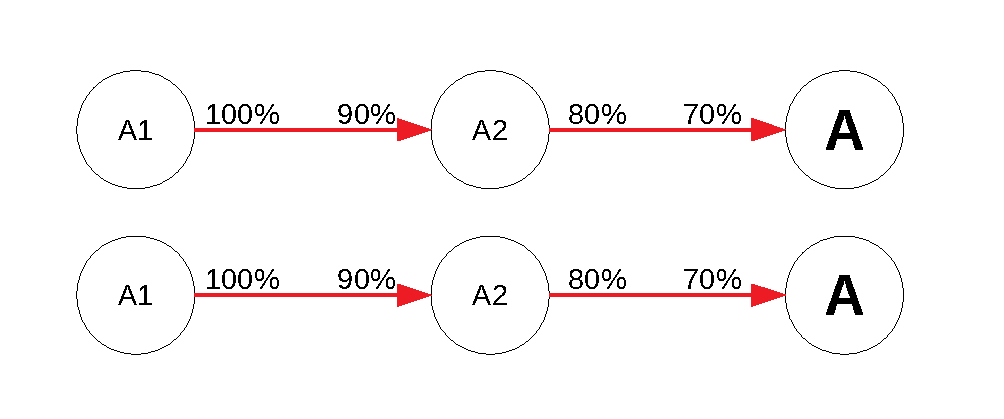
\includegraphics[scale=0.7]{MakeBatchPelda}
\caption{Példafeladat}
\label{MakeBatchPelda}
\end{center}
\end{figure}
Az új sorrend a \ref{tab:table1} táblázatban látható. Zárójelben pedig látható, hogy az ~\ref{MakeBatchPelda} ábrán melyik sorban lévő recepthez tartozik.
\begin{table}[H]
  \begin{center}
  	\caption{A taszkokhoz tartozó azonosítók}
  	\captionsetup[table]{skip=10pt}
    \label{tab:table1}
    \begin{tabular}{|c|c|}
      \textbf{Taszk} & \textbf{Azonosító} \\     
      \hline
      A1 (első) & 0\\
      A1 (második) & 1\\
      A2 (első) & 2\\
      A2 (második) & 3\\
    \end{tabular}
  \end{center}
\end{table}
Azt nem lehet megengedni, hogy a 0. azonosítóval rendelkező taszk és a 3. azonosítóval rendelkező taszk között él keletkezzen, mert nem ez a kettő taszk tartozik egymáshoz. A példafeladatban látható, hogy egy él kezdő taszkjának, és annak a taszknak, amelybe érkezik, az azonosítójuk különbsége éppen annyi, amennyi terméket gyártani szeretnénk. Jelen esetben kettő. 

\subsection{UpdateProfitBound függvény}
A függvény feladata, hogy kiszámolja az első S-gráfhoz tartozó korlátot, valamint minden egyes taszkhoz tartozó kapacitást is meghatározza. Legelső lépésben beállítja a taszkoknak az úgynevezett alap kapacitását. Ezt az alapján lehet meghatározni, hogy egyes berendezések, melyek a részfeladatot képesek elvégezni rendelkeznek-e kapacitással. Ezeket a bemeneti fájlból olvassa be a szoftver. Egy taszk kapacitását az összes, őt elvégezni képes taszk kapacitásának összege adja meg. Miután ez megtörtént a következő lépés a kezdő csomópontok, taszkok megkeresése. Ez 2 \textit{for} ciklus segítségével történik, amelyekben megvizsgáljuk, hogy az adott csomópont rendelkezik-e abba tartó, bementi éllel. Ha ilyen nincs akkor biztosak lehetünk benne, hogy az adott csomópont kezdő csomópont. Miután ezzel megvagyunk akkor megkeressük az előbb megtalált csomópontok szomszédjait. Ehhez egy \textbf{\textit{deque}} (double-ended queue), azaz kétvégű sort veszünk igénybe. Ennek előnye abban rejlik, hogy mind az elejéhez, mind a végéhez lehetséges elemet fűzni, illetve onnan eltávolítani. Ebbe a változóba tároljuk a kezdő csomópontok szomszédjait. Ismét két \textit{for} ciklus segítségével bejárjuk a taszkokat, amennyiben van köztük él, és még nem szerepel az adott taszk a \textbf{\textit{deque-ban}}, akkor beletesszük.

Mindezeket követően elérkezik az a rész, ahol a kapacitások felülvizsgálata következik. Egy \textit{while} ciklus segítségével minden \textbf{\textit{deque-ban}} szereplő elemet vizsgálunk addig, amíg az teljesen üressé nem válik. Először a \textbf{\textit{deque}} első elemét kivesszük belőle, majd egy \textit{for} ciklus segítségével ismét végighaladunk a taszkokon. Ha az éppen ciklusban lévő taszkból mutat él a \textbf{deque-ból} kivett taszkba, továbbá a taszknak, amiből az él indult, már korábban, a mostani függvény futása során felül lett vizsgálva a kapacitása, akkor lehet ellenőrizni a \textbf{\textit{deque-ból}} kivett taszk kapacitását. Ha az aktuálisan kiszámolt kapacitás nagyobb mint az eddigi, akkor a korábbi helyett az újat jelöljük ki a taszk kapacitásának. Ennek kiszámításhoz a 4. fejezetben bemutatott képletet kell használni.

Abban az esetben, ha a kezdeti taszk még nem lett ellenőrizve, akkor nem lehet megvizsgálni az éppen kiválasztott taszkot, ezért visszatesszük a \textbf{\textit{deque}} végére. Ha viszont lehetséges volt és végbe is ment az adott taszk felülvizsgálata, akkor megkeressük ennek a csomópontnak a szomszédjait és hozzáfűzzük a \textbf{\textit{deque}} végéhez.

A függvény utolsó szakaszában történik meg a profit korlát meghatározása, kiszámolása. A korlátot azoknak a taszkoknak a kapacitása adja meg, amelyek a termékek előtti utolsó részfeladatok. Ezek megtalálása úgy történik, hogy \textit{for} ciklus segítségével bejárjuk a termékeket, valamit a taszkokat is. Ha valamelyik taszkból indul él egy termékbe, akkor a taszk kapacitását megszorozzuk a termékből származó jövedelemmel.

\subsection{UpdateProfitBoundFromTask függvény}
Ez a függvény feladatában hasonlít az előző pontban bemutatott \textbf{UpdateProfitBound} metódushoz. A taszkokhoz tartozó kapacitást, valamint a korlátot kell meghatároznia. Különbséget abban lehet felfedezni, hogy ennek a függvénynek nem kell a teljes S-gráfot bejárnia, az összes kapacitást nem szükséges újraszámolnia, hanem csak a paraméterben megadott taszkokhoz, és az ezt követő taszkokhoz tartozó kapacitásokat kell újraszámolnia. Az ezt követő taszkokat úgy kell értelmezni, hogy a megadott taszk szomszédjait, valamint azoknak a szomszédjait (így tovább egészen addig, amíg létezik egy szomszéd taszk) kell átvizsgálni és szükség esetén megváltoztatni, módosítani a kapacitásukat.

Az előző pontban bemutatott függvénytől eltérően nem az S-gráf bemeneti node-jait, csomópontjait reprezentáló taszkokat kell először megkeresni, hanem a paraméterlistában átadottat, valamint annak közvetlen szomszédjait. Ehhez is a \textbf{\textit{deque-t}} veszünk igénybe. Legelsőnek az átadott taszk kerül bele, majd \textit{for} ciklus segítségével megkeresi annak szomszédjait, és ezeket is a \textbf{\textit{deque}} végéhez hozzáfűzi. Ezek után meg kell keresni a többi olyan taszkot is, amelyeknek a kapacitását újra át kell vizsgálni, és ha szükséges módosítást végezni. Azt követően, hogy a két végű sor tartalmazza az összes átvizsgálandó taszkot megtörténik a tényleges kapacitásmódosítás. Itt \textit{while} ciklus felhasználásával addig történik az ellenőrzés, amíg teljesen üressé válik a \textbf{\textit{deque}}. Ebből kivételre kerül a legelső elem, és megvizsgáljuk, hogy van-e ebbe tartó él, vagyis az S-gráf kezdő csomópontja vagy sem. Későbbiekben lesz szerepe ennek. Az éppen vizsgált taszk kapacitását átállítjuk nullára, majd a még hozzárendelhető berendezések kapacitásának összegét megkapja, mint új értéket. Amennyiben a taszknak nincs bejövő éle, akkor az imént meghatározott kapacitása megmarad, nincs szükség további ellenőrzésekre. Ellenben, ha van bemenő él, akkor még további feltételekre meg kell vizsgálni. Ha az a taszk, amelyből az él érkezik még nem ellenőrzött, akkor nem lehetséges a mostani taszk kapacitásának pontos meghatározása sem, ezért visszakerül a \textbf{\textit{deque}} végére. Azonban ha ellenőrzött a vizsgált taszkot megelőző részfeladat, akkor az előző pontban feltüntetett képlet szerint ki kell számolni a kapacitást. Ha ez nagyobb, mint a beállított, akkor ezt kapja meg a taszk új értékként. Ellenkező esetben pedig marad a már meglévő érték. Ezeket követően szükséges még egy \textit{for} ciklus segítségével végigmenni a taszkokon, annak érdekében, hogy ha létezik megtalálja az összes szomszédját az imént vizsgált taszknak. Ha talált ennek megfelelő taszkot akkor a \textbf{\textit{deque}} végéhez hozzáadjuk.

Utolsó lépés a függvényben a profit korlát kiszámítása. Ez teljes mértékben megegyezik az előző pontban szereplő függvény befejező lépésével. Az S-gráfon a termék előtt szereplő utolsó részfeladat kapacitása szükséges a korlát kiszámításához. Azért, hogy megtaláljuk ezt a taszkot szükség van arra, hogy két darab \textit{for} ciklus bejárja a termékeket és a taszkokat. Ha megtalálta akkor annak kapacitása és a terméken szerzett jövedelem szorzata megadja a korlátot.

\subsection{Egyéb új metódusok}
Az \textbf{IsProfitMaximization} függvény megadja, hogy a megoldó szoftver indításakor az új módszer került meghívásra parancssori paraméterek által. Olyan esetekben kerül meghívásra, amelyeket csak abban az esetben kell végrehajtani, ha az új $-$ taszkok párhuzamos végrehajtására alkalmas $-$ módszer lett meghívva. Például a futás végén a fájlba írásnál kapacitásokat csak ennél a módszernél akarunk kiírni.

A másik egyszerűbb függvény a \textbf{GetTaskCapacity}. Paraméterként egy részfeladat azonosítóját várja, és ez alapján visszaadja az adott taszkhoz tartozó kapacitást.

\section{Argumentum hozzáadás}
Az új módszer elkészítése miatt szükség volt két új argumentum hozzáadására. Az első \textbf{\textit{flexbatch}}, amely a \textbf{method} kapcsolóhoz tartozik, ezzel a megoldó módszert lehet kiválasztani. A második új argumentum a \textbf{\textit{profit\textunderscore max}}, amely a \textbf{obj} kapcsolóhoz tartozik, ez pedig a célfüggvényt reprezentálja.

\section{Megoldás fájlba írása}
Az új módszerrel kapcsolatos kapacitások kezelése eddig nem volt része a solver megoldó szoftvernek. Ez alól a fájlba történő kiírásuk sem kivétel, emiatt szükség volt a már meglévő kiírást elvégző függvény módosítására. A szóban lévő függvény a \textbf{WriteText}, amely \textbf{SGraph} típusú változót vár paraméterként.

Az eredetileg meglévő függvény a fájlba két elkülöníthető rész kiírását végezte. Az első az volt, amely megmutatta az éleket. Ebbe beletartozik mind a recept, mind az ütemezési élek csoportja. Ezenfelül még megjelenik itt egy időérték, amely azt mutatja, hogy az adott taszkot, amelyből az él kiindul mennyi idő alatt lehet befejezni, elvégezni. Továbbá a boundot, korlátot is itt írja ki a fájlba a függvény. A második fele pedig az elvégzett feladathoz tartozó Gantt diagramot jeleníti meg karakteres formában. Ez a rész megadja, hogy melyik taszkot, melyik berendezés végezi el és, hogy ez mikor történik.

Az említett két rész közé került az általam elkészített kapacitások kiírására szolgáló rész. Pontosabban, mivel az új módszer kapacitás és jövedelem szorzataként adja meg a korlátot ezért, a rész a kapacitások után jelenik ezentúl meg. Először a taszkok kapacitása kerül kiírásra, ezeket követik a termékek, amelyekhez az utolsó taszk kapacitása és a termékből származó jövedelem adja meg az értéket. A korlát kiszámítása a termékekhez tartozó értékek összeadásával történik.